\documentclass[12pt, a4paper]{article}
\usepackage[lmargin =0.5 in, 
rmargin=0.5in, 
tmargin=1in,
bmargin=0.5in]{geometry}
\geometry{letterpaper}
\usepackage{tikz-cd}
\usepackage{amsmath}
\usepackage{amssymb}
\usepackage{blindtext}
\usepackage{titlesec}
\usepackage{enumitem}
\usepackage{fancyhdr}
\usepackage{amsthm}
\usepackage{graphicx}
\usepackage{cool}
\usepackage{thmtools}
\usepackage{hyperref}
\usepackage{subcaption}
\usepackage{tabu}
\usepackage{biblatex}
\usepackage{float}
\graphicspath{}					%path to an image

%-------- sexy font ------------%
%\usepackage{libertine}
%\usepackage{libertinust1math}

%\usepackage{mlmodern}				% very nice and classic
%\usepackage[utopia]{mathdesign}
%\usepackage[T1]{fontenc}


\usepackage{mlmodern}
\usepackage{eulervm}
%\usepackage{tgtermes} 				%times new roman
%-------- sexy font ------------%


% Problem Styles
%====================================================================%


\newtheorem{problem}{Problem}


\theoremstyle{definition}
\newtheorem{thm}{Theorem}
\newtheorem{lemma}{Lemma}
\newtheorem{prop}{Proposition}
\newtheorem{cor}{Corollary}
\newtheorem{fact}{Fact}
\newtheorem{defn}{Definition}
\newtheorem{example}{Example}
\newtheorem{question}{Question}

\newtheorem{manualprobleminner}{Problem}

\newenvironment{manualproblem}[1]{%
	\renewcommand\themanualprobleminner{#1}%
	\manualprobleminner
}{\endmanualprobleminner}

\newcommand{\penum}{ \begin{enumerate}[label=\bf(\alph*), leftmargin=0pt]}
	\newcommand{\epenum}{ \end{enumerate} }

% Math fonts shortcuts
%====================================================================%

\newcommand{\ring}{\mathcal{R}}
\newcommand{\N}{\mathbb{N}}                           % Natural numbers
\newcommand{\Z}{\mathbb{Z}}                           % Integers
\newcommand{\R}{\mathbb{R}}                           % Real numbers
\newcommand{\C}{\mathbb{C}}                           % Complex numbers
\newcommand{\F}{\mathbb{F}}                           % Arbitrary field
\newcommand{\Q}{\mathbb{Q}}                           % Arbitrary field
\newcommand{\PP}{\mathcal{P}}                         % Partition
\newcommand{\M}{\mathcal{M}}                         % Mathcal M
\newcommand{\eL}{\mathcal{L}}                         % Mathcal L
\newcommand{\T}{\mathbb{T}}                         % Mathcal T
\newcommand{\U}{\mathcal{U}}                         % Mathcal U\\
\newcommand{\V}{\mathcal{V}}                         % Mathcal V

% symbol shortcuts
%====================================================================%

\newcommand{\bd}{\partial}
\newcommand{\grad}{\nabla}
\newcommand{\lam}{\lambda}
\newcommand{\imp}{\implies}
\newcommand{\all}{\forall}
\newcommand{\exs}{\exists}
\newcommand{\delt}{\delta}
\newcommand{\ep}{\varepsilon}
\newcommand{\ra}{\rightarrow}
\newcommand{\vph}{\varphi}

\newcommand{\ol}{\overline}
\newcommand{\f}{\frac}
\newcommand{\lf}{\lfrac}
\newcommand{\df}{\dfrac}

% bracketting shortcuts
%====================================================================%
\newcommand{\abs}[1]{\left| #1 \right|}
\newcommand{\babs}[1]{\Big|#1\Big|}
\newcommand{\bound}{\Big|}
\newcommand{\BB}[1]{\left(#1\right)}
\newcommand{\dd}{\mathrm{d}}
\newcommand{\artanh}{\mathrm{artanh}}
\newcommand{\Med}{\mathrm{Med}}
\newcommand{\Cov}{\mathrm{Cov}}
\newcommand{\Corr}{\mathrm{Corr}}
\newcommand{\tr}{\mathrm{tr}}
\newcommand{\Range}[1]{\mathrm{range}(#1)}
\newcommand{\Null}[1]{\mathrm{null}(#1)}
\newcommand{\lan}{\langle}
\newcommand{\ran}{\rangle}
\newcommand{\norm}[1]{\left\lVert#1\right\rVert}
\newcommand{\inn}[1]{\lan#1\ran}
\newcommand{\op}[1]{\operatorname{#1}}
\newcommand{\bmat}[1]{\begin{bmatrix}#1\end{bmatrix}}
\newcommand{\pmat}[1]{\begin{pmatrix}#1\end{pmatrix}}
\newcommand{\vmat}[1]{\begin{vmatrix}#1\end{vmatrix}}

\newcommand{\amogus}{{\bigcap}\kern-0.8em\raisebox{0.3ex}{$\subset$}}
\newcommand{\Note}{\textbf{Note: }}
\newcommand{\Aside}{{\bf Aside: }}
%restriction
%\newcommand{\op}[1]{\operatorname{#1}}
%\newcommand{\done}{$$\mathcal{QED}$$}

%====================================================================%


\setlength{\parindent}{0pt}      	% No paragraph indentations
\pagestyle{fancy}
\fancyhf{}							% fancy header

\setcounter{secnumdepth}{0}			% sections are numbered but numbers do not appear
\setcounter{tocdepth}{2} 			% no subsubsections in toc

%template
%====================================================================%
%\begin{manualproblem}{1}
%Spivak.
%\end{manualproblem}

%\begin{proof}[Solution]
%\end{proof}

%----------- or -----------%

%\begin{problem} 		
%\end{problem}	

%\penum
%	\item
%\epenum
%====================================================================%


\newcommand{\Course}{ECO462}
\newcommand{\hwNumber}{1}

%preamble

\title{ECO462A1}
\author{Ahmed }
\date{\today}
\lhead{\Course A\hwNumber}
\rhead{\thepage}
%\cfoot{\thepage}


%====================================================================%
\begin{document}
	
	\begin{titlepage}
		\begin{center}
			\vspace*{1cm}
			
			\huge \textbf{VXO and VIX}
			
			\vspace{0.5cm}

			
			\vspace{1.5cm}
			
			\small \textbf{Ahmed Abd-Elrazig, Alexander Neagoe}\\
			\vspace{5cm}
			
\includegraphics[width=0.6\textwidth]{UofT.png}
			\vspace{5cm}
			
			ECO462\\
			Christian Gourieroux\\
			University of Toronto\\
			October 22 2023
			
		\end{center}
	\end{titlepage}
\section{Analysis}
\begin{problem}
\end{problem}
\quad CBOE, or Chicago Board Options Exchange is an options exchange located in Chicago, responsible for the creation of the VIX, a volatility index. In the same way a market index is meant to capture the average behaviour of the market via a market portfolio, a volatility index measures the market's implied volatility. 
Rather than measuring the true volatility, which often may be too difficult to compute, CBOE opted to estimate the 30 day implied volatility, which is the market's expectation of volatility over a period of 30 days. This is done by computing the implied volatility of calls and puts which expire within 23-37 days, on a fixed portfolio of stocks. The value of the VIX is computed using the following formula: 
$$\sigma^2 =\frac{2}{T} \sum_i \frac{\Delta K_i}{K_i^2}e^{RT} Q(K_i) - \frac{1}{T} \left[\frac{F}{K_0} - 1  \right]^2. \quad [1] $$
Where: 
\penum
\item  $T$ is the time to expiration in minutes
\item $F$ is the forward index level derived from index option prices
\item $K_0$ is the first strike price below forward index level, $F$
\item $K_i$ is strike price of the $i'th$ out of the money option
\item $\Delta K_i = \frac{K_{i+1} - K_{i-1}}{2}$
\item $R$ is the risk free interest rate
\item $Q(K_i)$, is the midpoint of the bid-ask spread on option with strike $K_i$.
\epenum
The $VIX$ is defined to be $100 \times \sigma$, using the $S \&P 500$, while the VXO is defined on the $S\&P 100$. 
\begin{problem}
\end{problem}
\quad We plot the time evolution of the closing price of the VIX index and VXO index shown in Figure 1 and Figure 2 respectively. As volatility indices, we expect them to attain higher values during times where the market's implied volatility is high, such as during a recession or economic crisis. We see that in early 2020, and in 2008 that both the VIX and VXO. 
However we can also see that the market volatility fluctuates greatly yet does not have any clear trends.  In between recessions, the volatility indicated by the VIX could be the growth of the market. 
\begin{problem}
\end{problem}
\quad We first discuss the VIX. We refer to Table 1. for the moments of the distribution. 
We see that VIX price has positive skew, and a kurtosis of $8.29$. This suggests that the distribution of the price greatly diverges from a normal distribution, which has $0$ skew and a kurtosis of $3$. This observation is reflected in the Q-Q plot of price as shown in figure 11. The plot shows that the distribution of price greatly diverges from a normal distribution. However Figure 13 shows that the price more closely distributes to a fitted Lognormal distribution. This is reinforced by noting that lognormal distributions always have a positive skew. Turning our attention to the VIX returns, we see that the distribution of returns has a skewness of $0.316$ and a kurtosis of $3.67$, which is relatively closer to a normal distribution.
We observe that in Figure 7, the Q-Q plot of returns, that the returns almost distribute normally, except we note that the tails appear to contain more mass than in a normal distribution. 
If we think of the VIX as a stock, this is in line with what we would expect; lognormally distributed price, normally distributed returns.
\\

\quad We now focus on the VXO. The VXO price distribution, similarly to the VIX has positive skewness. Hence it can not come from a normal distribution. Inspecting the Q-Q plot against a normal as in Figure 12, we can obtain the same result. When we compare it to a Lognormal distribution using a Q-Q plot in Figure 14 we see that a Lognormal better describes it. However the right tail appears to be larger than a typical lognormal. This could be explained by the fact that the VXO is comprised of $100$ stocks as opposed to $500$, a smaller sample has a higher variance. The VXO returns are closer to normal than a lognormal, which is indicated by a skewness of $0.0360$ and a kurtosis of $3.32$. Once again this is what we expect if we view the VXO as a stock; lognormal price and normal returns. 

\begin{problem}
\end{problem}
\quad As one discerns from the graphical representation, the VIX index manifests two pronounced intervals of heightened volatility. The first notable surge aligns with the financial tumult of 2008, a period synonymous with severe market dislocation and pervasive uncertainty. The second significant elevation commences at the advent of 2020, concomitant with the onset of the global pandemic. This escalation underscores the profound levels of market uncertainty and the apprehension that characterized that epoch. These pivotal spikes, emblematic of broader economic distress and market trepidation, serve as poignant reminders of the VIX's capacity to encapsulate the prevailing market sentiment and its underlying volatility".
\\

This appears to be indicative of an efficient market, given that it displays no discernible patterns. This observation aligns with the Efficient Market Hypothesis, drawing parallels with the random walk theory which posits that price movements are unpredictable and random.
\\

\quad Given that market participants actively trade the VIX, it's logical for them to seek ways to hedge against its volatility. To elaborate, consider the mechanics of VIX ETNs (Exchange Traded Notes). These instruments necessitate the rolling of VIX future contracts. Often, these futures are in contango, which means as the contracts approach maturity, their spot price decreases. This implies a significant cost when rolling these futures, causing all VIX ETNs to have a persistent downward trajectory.
\\

\quad This situation provides a strategic opportunity for institutional investors. By shorting VIX futures to ETN providers, they can capture the risk premium, given the inevitable decline of these ETNs. This strategy has made it popular among major institutional players to maintain consistent short positions on VIX futures.
\\

\quad However, with any investment strategy, there's a need for hedging against potential adverse movements. For these institutions, a safeguard against significant losses from their short VIX positions becomes crucial. The ideal hedge in this case would be to take a long position on the volatility of VIX. This ensures that while they earn a consistent risk premium, they're also protected against substantial losses.
\\

\quad Recognizing this need, the CBOE introduced the VVIX index, which monitors the implied volatility of the VIX. Furthermore, market participants can also engage in trading volatility swaps on the VIX to manage their risk.
\begin{problem}
\end{problem}
\quad Before the change in 2003, the VIX was calculated using at-the-money S\&P 100 (OEX) option prices, while after the change, it was calculated using a wider set of S\&P 500 (SPX) option prices, both puts and calls. This change was made to provide a more accurate and comprehensive measure of market volatility.
\\

The reasons for the 2003 change include:
\begin{enumerate}[label = \roman*.]
\item Broader Market Representation: The S\&P 500 represents a much broader segment of the market than the S\&P 100, which means that VIX based on SPX options would be more representative of the overall market sentiment.

\item Enhanced Sensitivity: By using a wide range of strike prices, rather than just at-the-money options, the new methodology became more sensitive to changes in market sentiment.

\item Consistency and Smoothness: The new methodology, which uses a wide range of option prices, tends to produce a smoother and more consistent VIX series.

\item More Comprehensive Measure: The new methodology incorporated both put and call option prices, providing a more comprehensive measure of volatility expectations.

\end{enumerate}

\quad The VXO and the VIX are both volatility indices, but they are calculated using different underlying assets. The VXO, originally known as VIX, was based on the S\&P 100 index option prices, whereas the modern VIX is based on the S\&P 500 index option prices. The reasons for computing both in parallel for some time can be understood in the following context:

\begin{enumerate}[label = \roman*.]
\item Historical Comparisons: Given that the original VIX (now VXO) had a historical series of data, it was useful to continue its calculation to allow market participants to make longitudinal comparisons and analyze trends over time.

\item Different Market Segments: The S\&P 100 (OEX) represents a narrower segment of the market than the S\&P 500. Some market participants may have preferred to track the volatility of the more concentrated OEX, while others may have opted for the broader representation of the SPX.

\item Transition Period: When introducing a new methodology or basis for a widely followed index, there is often a period of coexistence to allow market participants to adjust to the new index and understand the differences between the old and new methodologies.

\item Diverse Derivative Products: Different volatility products might have been tied to the VXO and VIX, respectively. By computing both, the Chicago Board Options Exchange (CBOE) could cater to a broader set of market needs.

\item Academic and Research Purposes: For empirical research, having both indices provides a richer dataset to test hypotheses about market volatility, risk perceptions, and the relationship between broad and narrow market indices.

\end{enumerate}

\quad Over time, as the market adapted and the new VIX based on the S\&P 500 became more widely accepted, the importance of VXO diminished. However, during the parallel computation period, it was instrumental in offering a diverse perspective on market volatility and catering to the varied needs of traders, researchers, and other market participants.
\begin{problem}
\end{problem}
Pre-Pandemic Levels: Before the news of the pandemic started unsettling global markets, the VIX was relatively tame. On January 2, 2020, the VIX opened at roughly 13.46, well within the lower end of its historical range.
\begin{enumerate}[label=\roman*.]
\item Initial Escalation: By February 21, 2020, the VIX had crept up to an opening level of about 15.87. However, within a week, by February 28, it had more than doubled to open at 39.62. This represented a staggering increase of approximately 150% in just one week.

\item March Elevation: March 2020 was when the gravity of the pandemic truly hit financial markets. The VIX continued its rapid ascent:

\item March 9: Opened at 54.47.

\item March 12: Jumped to open at 64.40.

\item March 16: Peaked at an opening level of 82.69, a level not seen since the financial crisis in 2008.

To put this in perspective, from the beginning of March to its peak on March 16, the VIX experienced an increase of more than 300% from its end-February levels.

Post-Peak Moderation: After the mid-March peak, the VIX started retreating but remained elevated:

End of March: It was still hovering around the 50s.

By the end of April: It had declined to the high 30s but was still about three times its January levels.

\end{enumerate}
\quad Rate of Change: The speed of this VIX spike was unparalleled. The month-over-month rate of change, especially from February to March 2020, was one of the fastest and most significant in the VIX's history.
\\

\quad To give context, such rapid and extreme VIX movements are unusual. They typically only occur during times of profound market stress, such as the financial crisis of 2008. The VIX, in its role as the market's "fear gauge," vividly illustrated the swift shift from complacency in January to near-panic in March.
\\

\quad The subsequent moderation in the VIX, while reflective of some return of confidence due to central bank and government interventions, still indicated a market on edge and uncertain about the future. 
\newpage
\section{Figures and Tables:}
\begin{table}[H]
	\centering
	\begin{tabu}to \textwidth {X[c]X[c]}
		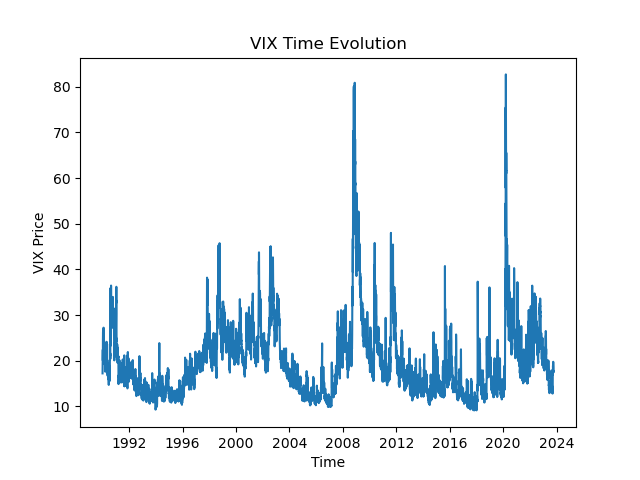
\includegraphics[width=75mm]{VIX Time Evolution.png}\captionof{figure}{VIX Time Evolution} 
		&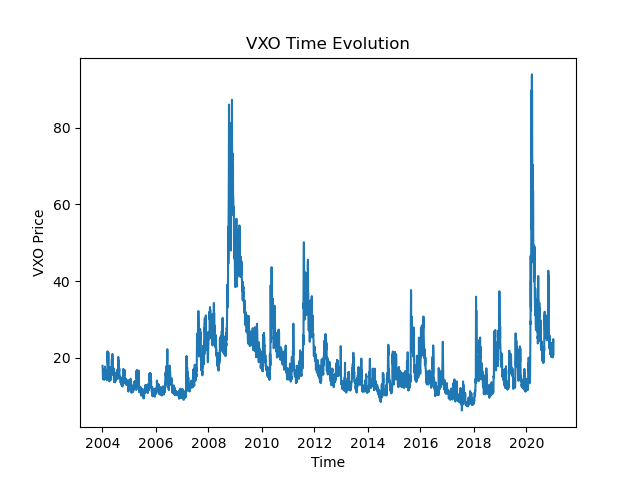
\includegraphics[width=75mm]{VXO Time Evolution.png}\captionof{figure}{VXO Time Evolution} 
		\\ 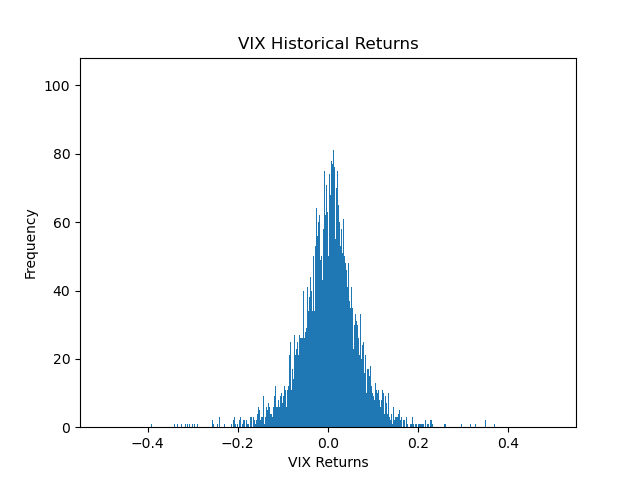
\includegraphics[width=75mm]{VIX Historical Returns.png}\captionof{figure}{VIX Historical Returns} 
		&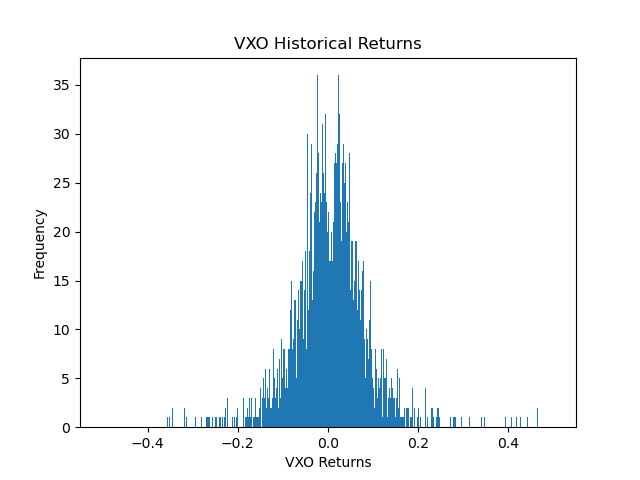
\includegraphics[width=75mm]{VXO Historical Returns}\captionof{figure}{VXO Historical Returns} \\
		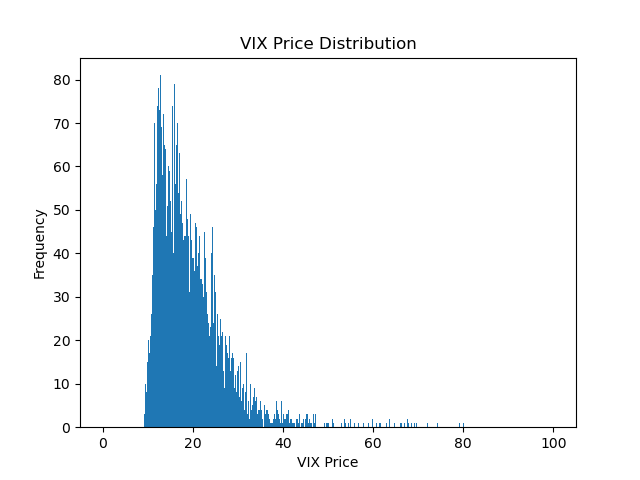
\includegraphics[width = 75mm]{VIX Price.png}\captionof{figure}{VIX Price Distribution}
		& 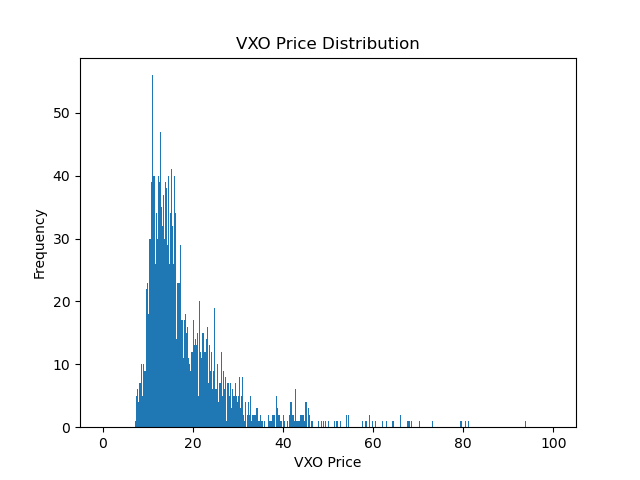
\includegraphics[width = 75mm]{VXO Price.png}\captionof{figure}{VXO Price Distribution}
	\end{tabu}
\end{table}

\begin{table}[H]
	\centering
	\begin{tabu}to \textwidth {X[c]X[c]}
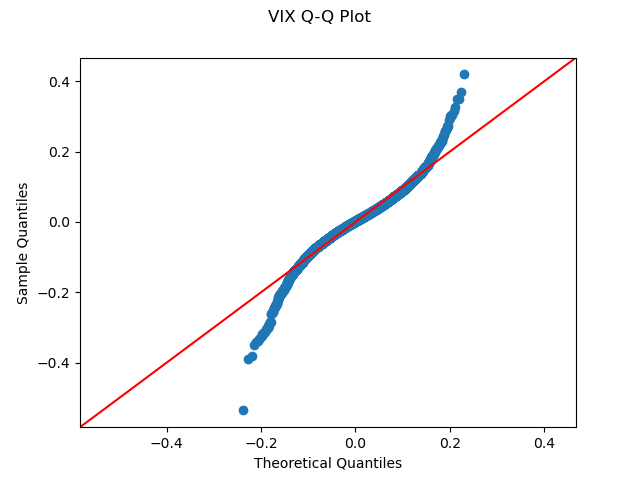
\includegraphics[width=75mm]{VIX Q-Q Plot.png}\captionof{figure}{VIX Returns Q-Q Plot} &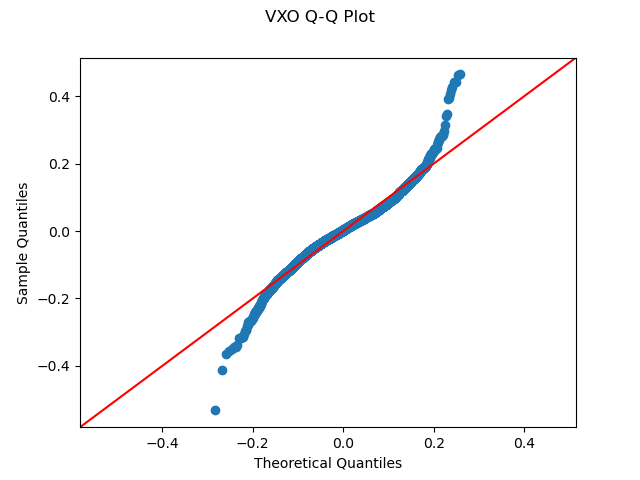
\includegraphics[width=75mm]{VXO Q-Q Plot.png}\captionof{figure}{VXO Returns Q-Q Plot} \\
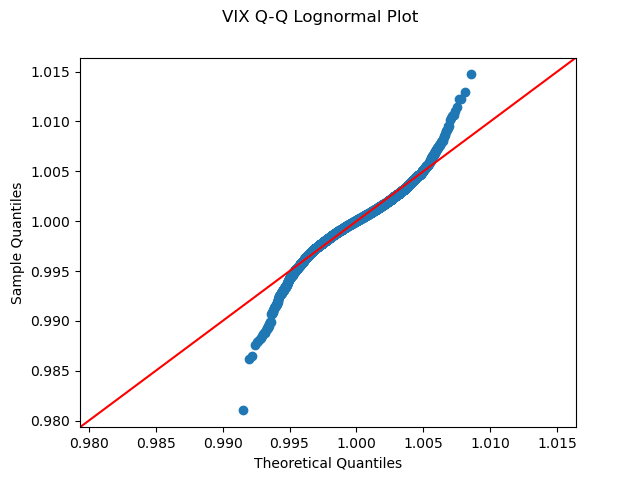
\includegraphics[width=75mm]{VIX Q-Q Plot Log.png}\captionof{figure}{VIX Returns Q-Q Plot Log} &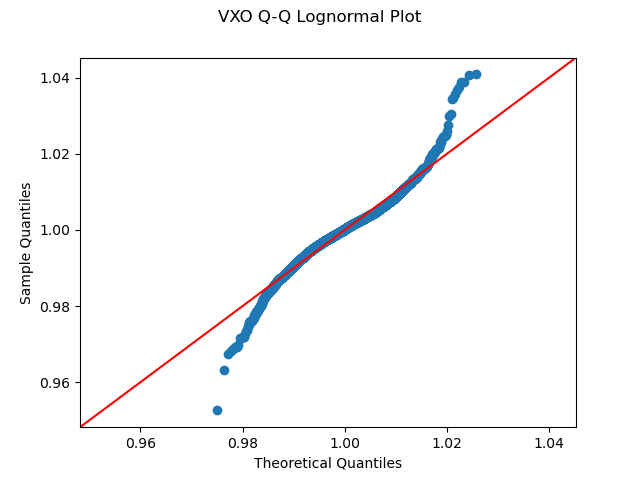
\includegraphics[width=75mm]{VXO Q-Q Plot Log.png}\captionof{figure}{VXO Returns Q-Q Plot Log} \\
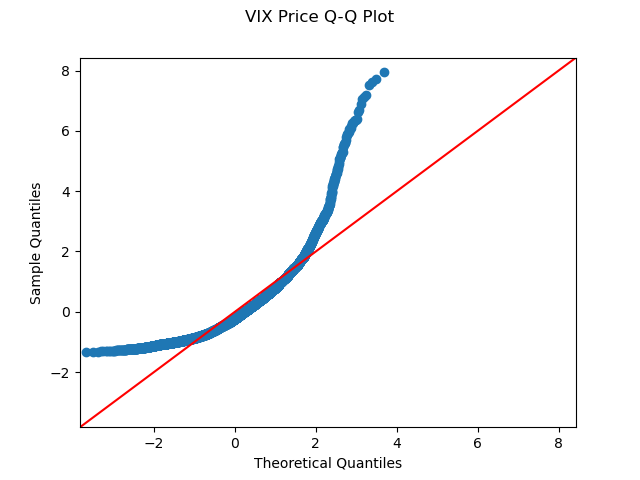
\includegraphics[width=75mm]{VIX Price Q-Q Plot.png}\captionof{figure}{VIX Price Q-Q Plot} &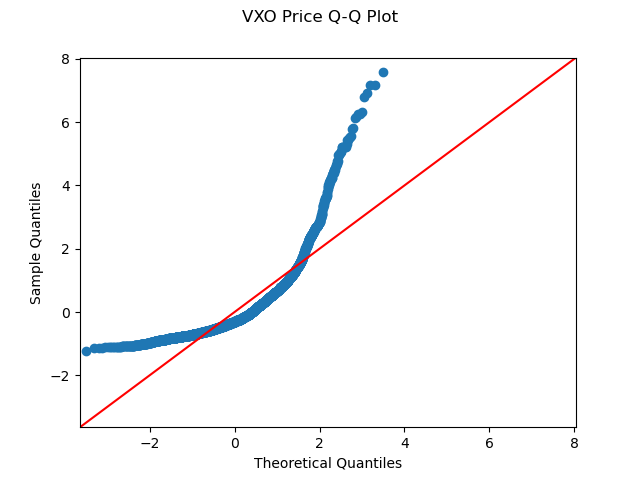
\includegraphics[width=75mm]{VXO Price Q-Q Plot.png}\captionof{figure}{VXO Price Q-Q Plot} \\
	\end{tabu}
\end{table} 

\begin{table}[H]
	\centering
	\begin{tabu}to \textwidth {X[c]X[c]}

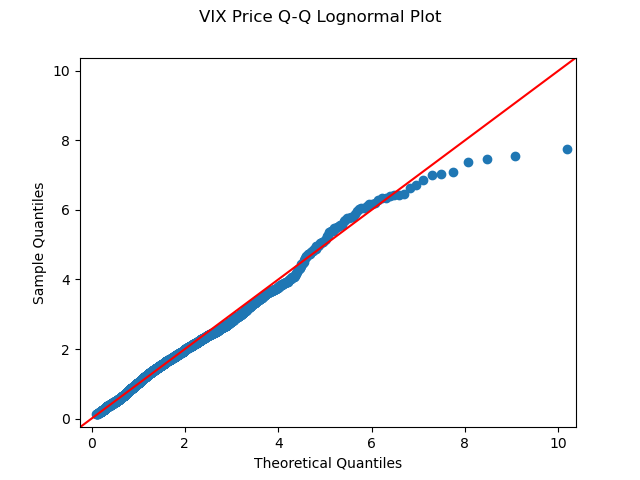
\includegraphics[width=75mm]{VIX Price Q-Q Plot Log.png}\captionof{figure}{VIX Price Q-Q Plot Log} &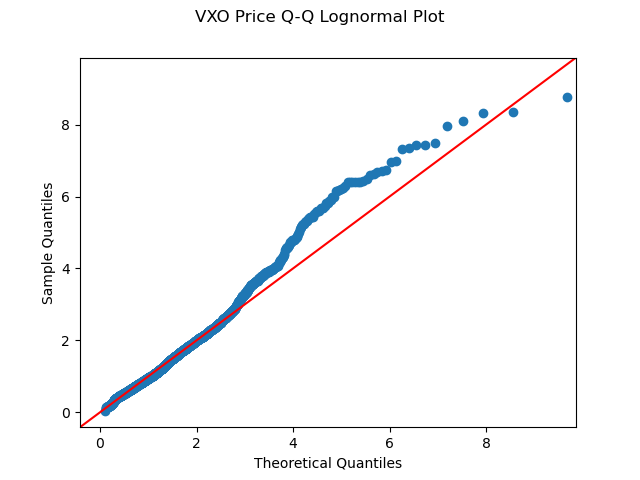
\includegraphics[width=75mm]{VXO Price Q-Q Plot Log.png}\captionof{figure}{VXO Price Q-Q Plot Log} \\ 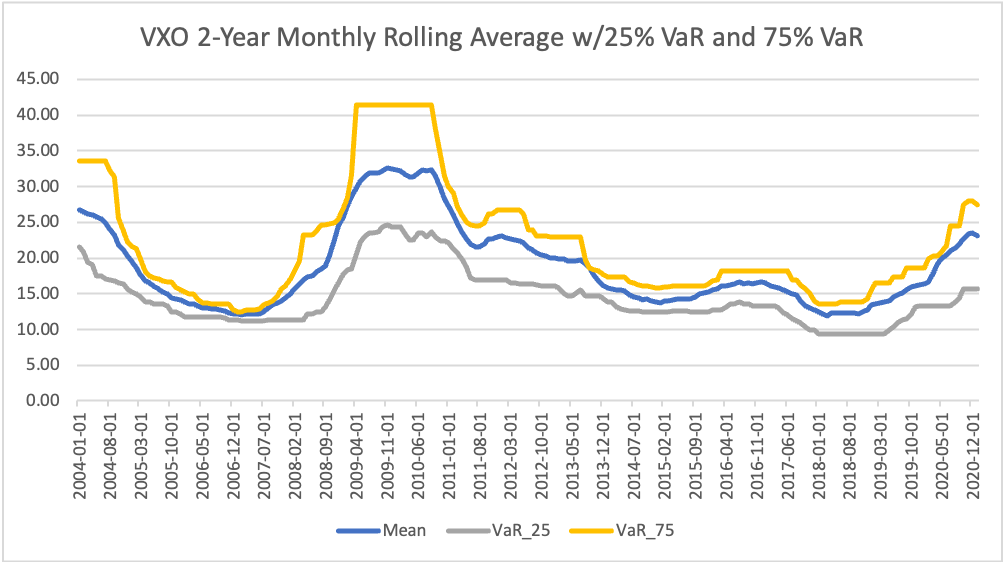
\includegraphics[width=75mm]{eco462A1Q4a.png}\captionof{figure}{VaR, 25\%,75 \% } & 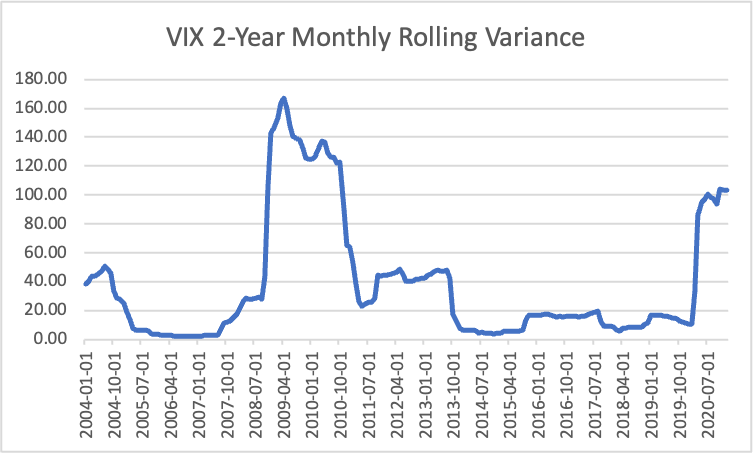
\includegraphics[width=75mm]{eco462A1Q4b.png}\captionof{figure}{VIX bi-monthly rolling variance}\\
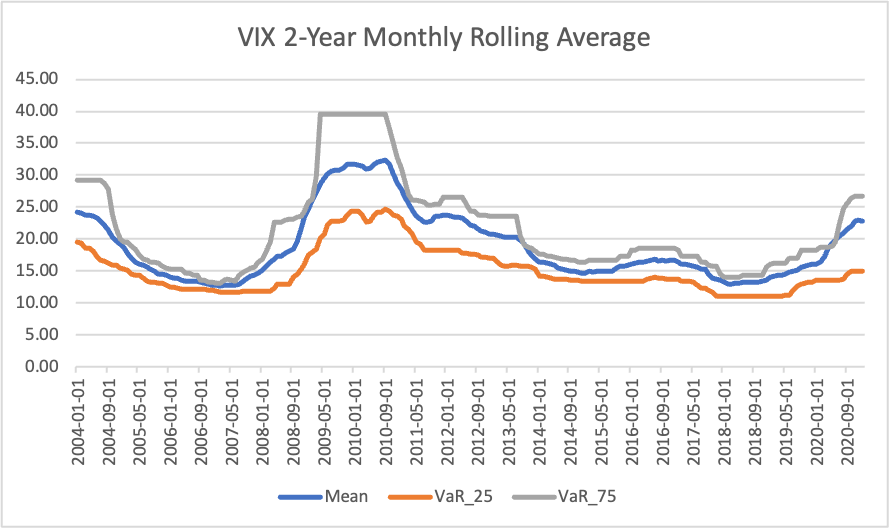
\includegraphics[width=75mm]{eco462A1Q4c.png}\captionof{figure}{VaR, bi-monthly rolling avg.}
	\end{tabu}
\end{table} 

\begin{table}[h!]
	\caption{Moments}
	\centering
	\begin{tabular}{c c c c c}
		\hline \hline
		Index & Mean & Std. Dev. & Skewness & Kurtosis\\
		\hline
		VIX returns & -0.00220 & 0.0654 & 0.316 & 3.67\\
		VIX Price & 19.61 & 7.92 & 2.14 & 8.29\\
		VXO returns & -0.0339 &0.0820 & 0.0360 & 3.32\\
		VXO Price & 18.60 & 9.91 & 2.729 &2.72s 
	\end{tabular}
\end{table}
\newpage 
\section{References}
	 [1] Volatility Index Methodology. Chicago Board Options Exchange. (n.d.).\newline  https://cdn.cboe.com/api/global/us\_indices/governance/Volatility\_Index\_Methodology\_Cboe\_Volatility\_Index. \\ pdf 

\end{document}
